\documentclass[PICOReport.tex]{subfiles}

\begin{document}

\begin{figure*}
%\vskip-3cm
\begin{center}
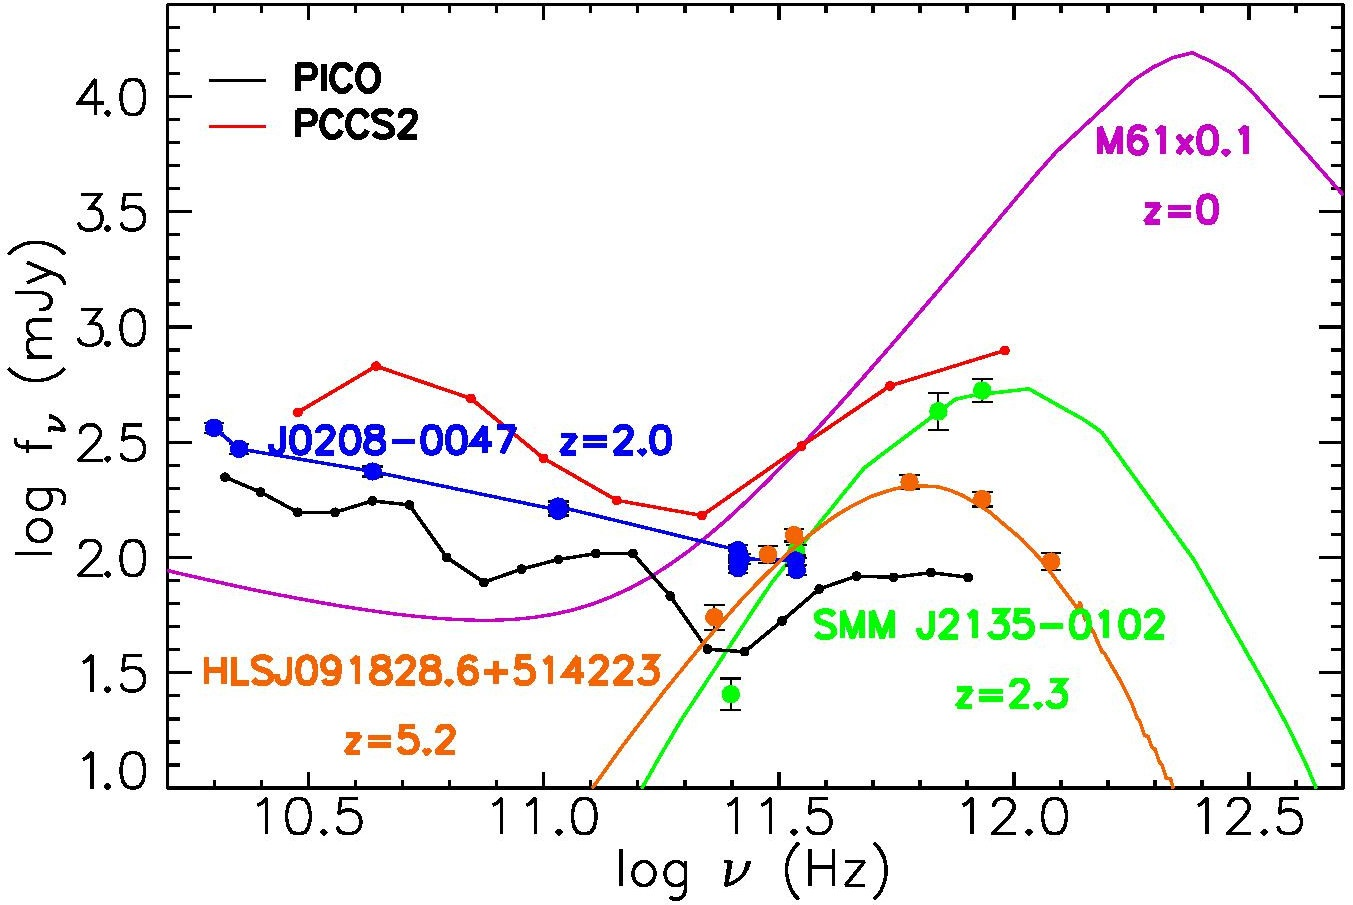
\includegraphics[width=0.48\columnwidth, trim={0 0 0 0cm}, clip]{images/fig_SED3_PICO.jpg}
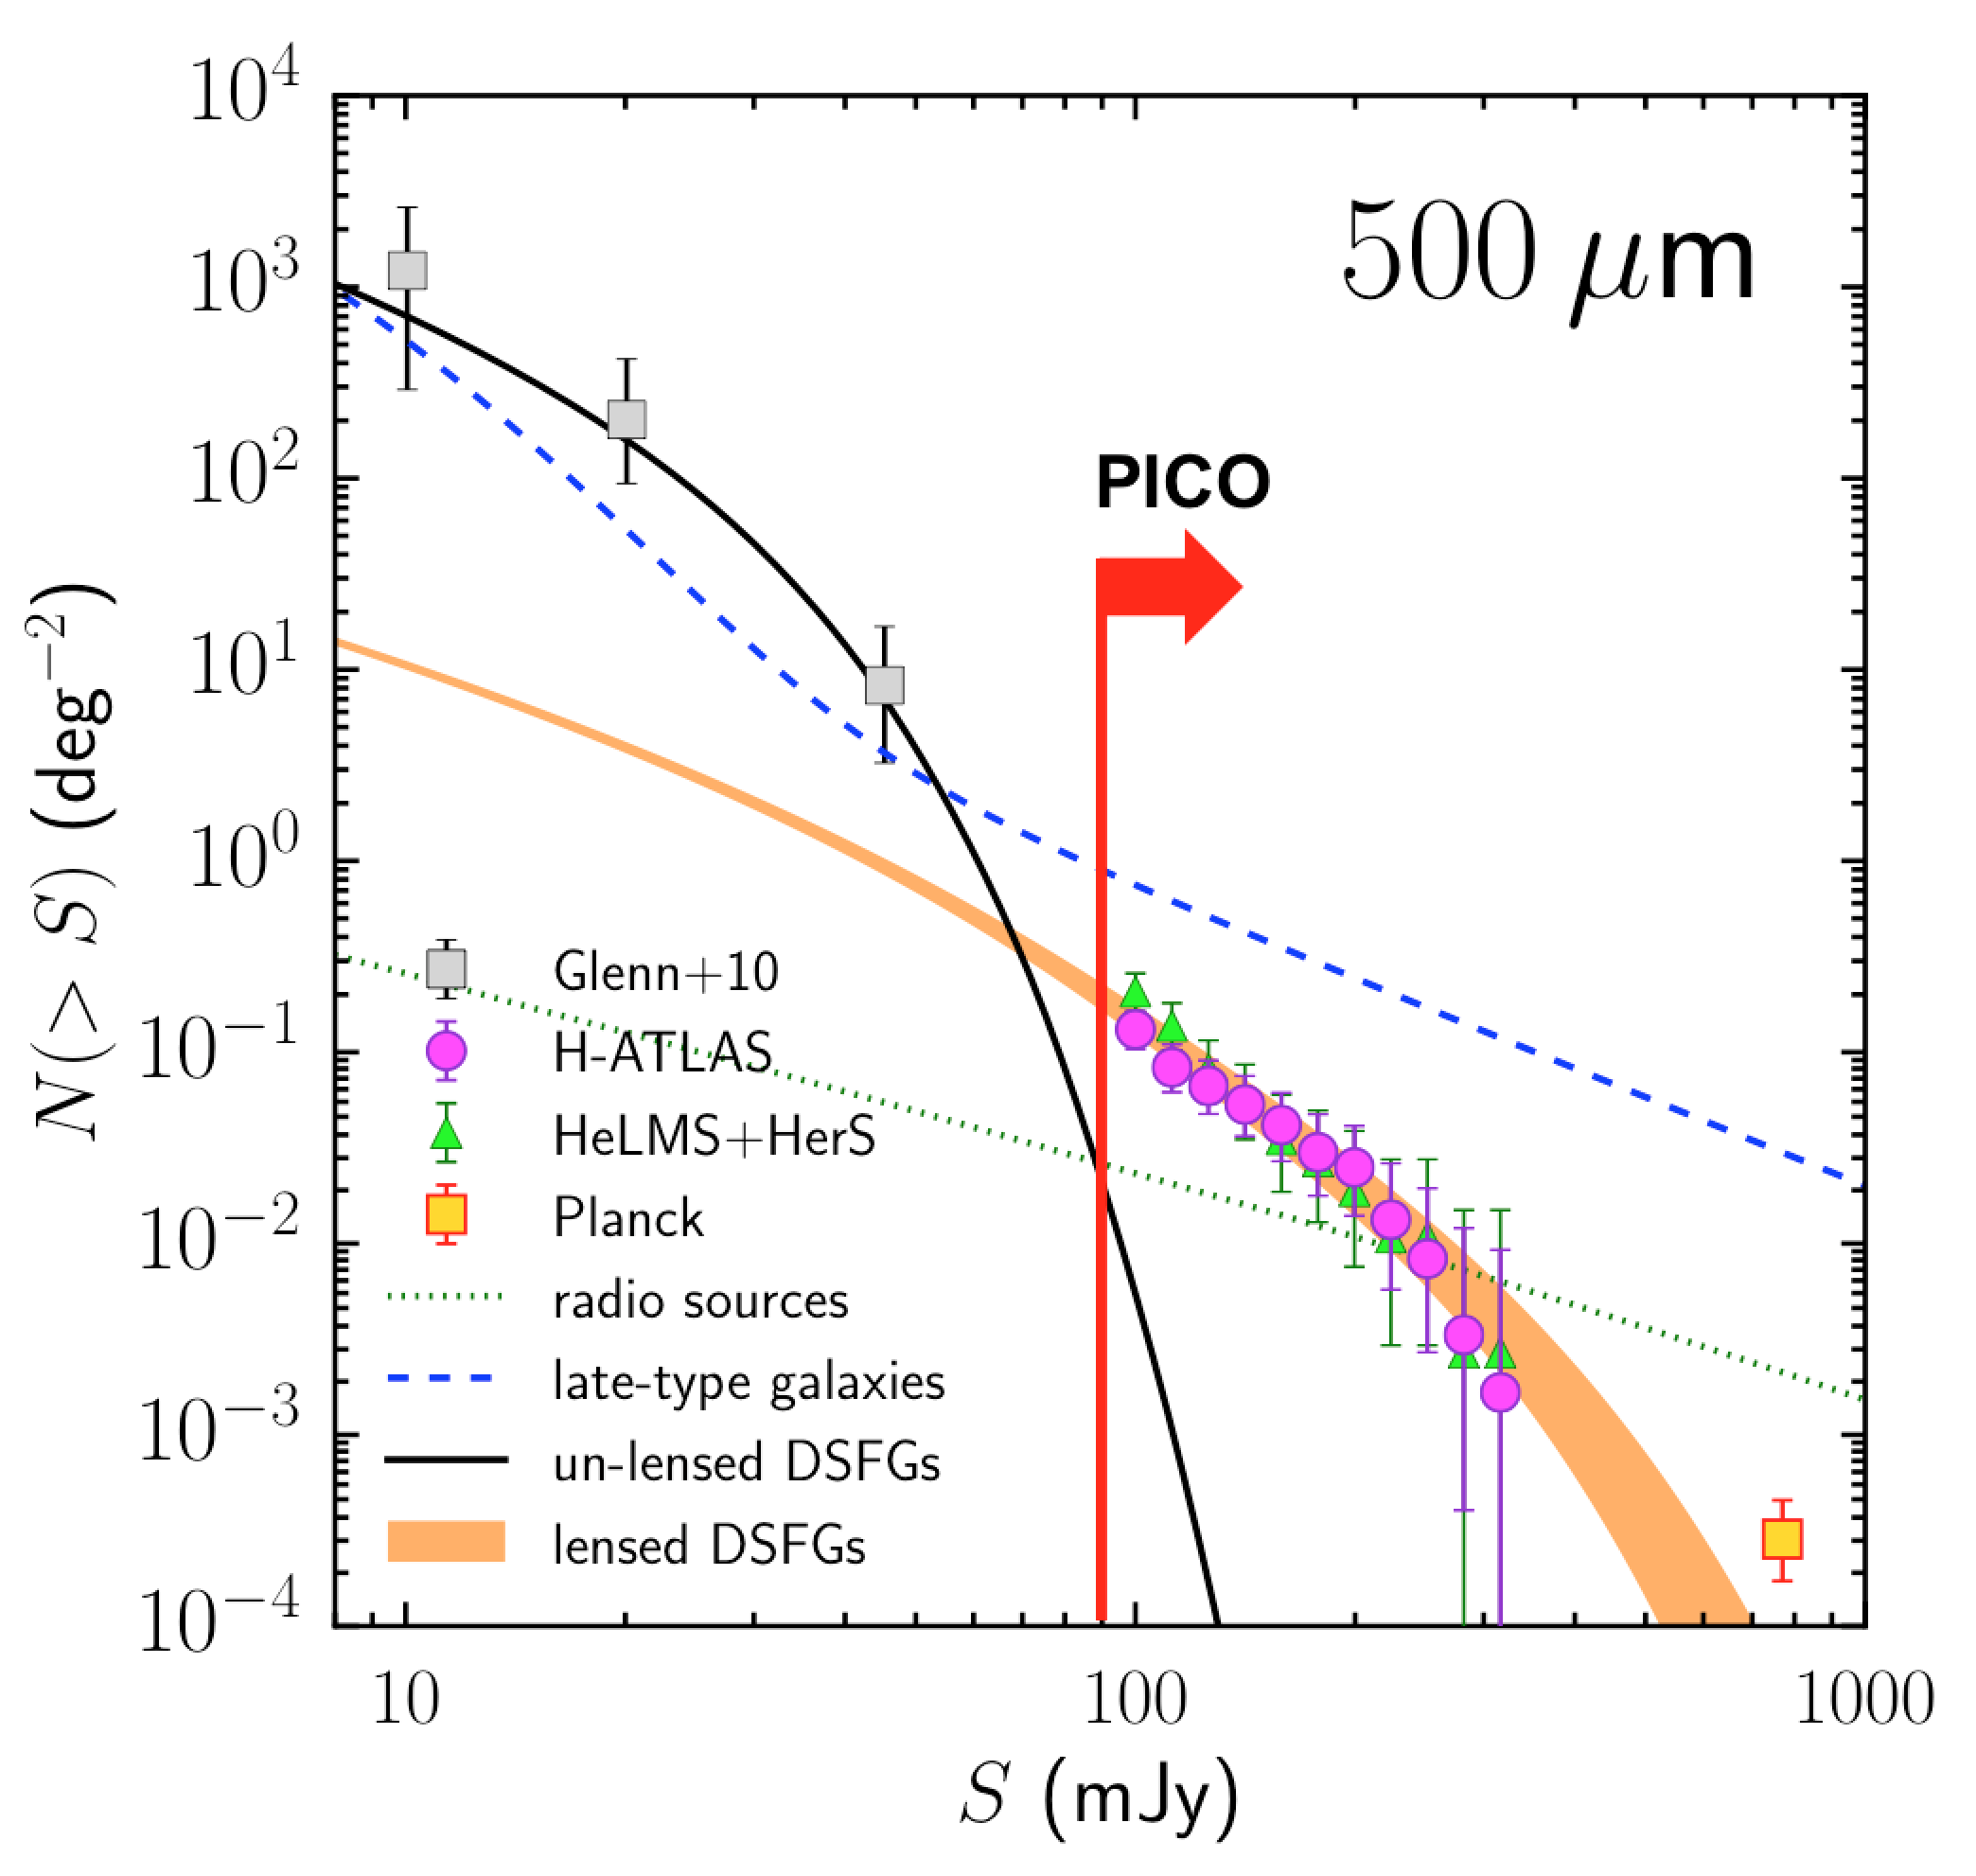
\includegraphics[width=0.48\columnwidth, height=5.5truecm, trim={0 0 0 0cm}, clip]{images/NgtF_500micron.png}
\caption{\textbf{Left panel.} Examples of SEDs of extragalactic sources detectable by PICO,
compared with its point source detection limits (solid black line). The SED of M\,61 has been scaled down by a
factor of 10. The 90\% completeness limits of the Second \textit{Planck} Catalogue of Compact Sources (PCCS2; \cite{PCCS2})
are also shown.  \textbf{Right panel.} Integral counts of the various populations of extragalactic sources at
$500\,\mu$m as determined by \textit{Herschel} surveys. The vertical red line shows the estimated PICO detection limit.}
\label{fig:SED3}
\end{center}
\end{figure*}

\subsubsection{Point extragalactic sources in the PICO frequency range}

As illustrated by the left panel of Fig.\,\ref{fig:SED3}, at $\lambda \simgt
\hbox{few\, mm}$ the  dominant extragalactic population are blazars
(flat-spectrum radio quasars, FSRQs, and BL Lacs), typically at $z\simgt 1$;
the solid blue line shows an example. At shorter wavelengths dusty galaxies
take over. The brightest sources in this spectral range are nearby
star-forming galaxies like M\,61. PICO will also see the brightest high-$z$
sub-mm sources which, due to the ``magnification bias'', are those whose flux
density is boosted by strong gravitational lensing.

\textit{Herschel} surveys have shown that, at $500\,\mu$m (600\,GHz), about
20\% of galaxies  at the PICO detection limit are strongly lensed (right panel
of Fig.\,\ref{fig:SED3}). This is an extraordinary selection efficiency: for
comparison, the fraction of strongly lensed galaxies is of $\sim 10^{-3}$ in
all other frequency bands where searches have been carried out. Also, these
galaxies have sub-mm colors substantially different from those of the other
extragalactic populations and are therefore very easily singled out
\cite{Negrello2017lensed}.

PICO will detect several thousands strongly lensed galaxies. Objects like the
$z=4$ source  HLSJ$091828.6+514223$ (left panel of Fig.\,\ref{fig:SED3};
\cite{Combes2012}) would be detectable by PICO up to extreme redshifts
($z>10$).

The availability of thousands of strongly lensed galaxies opens exciting
prospects both  on the astrophysical and on the cosmological side (cf., e.g.,
ref. \cite{Treu2010}). Compared to searches in other wavebands, PICO detections
will extend to much higher redshift sources \cite[most optically-selected
strongly lensed galaxies are at $z<1$, cf. Fig.\,7 of ref. ][]{Treu2010} and
will pick up the rare most extreme amplifications, thanks to its all sky
coverage: the magnification factors, $\mu$, of ``\textit{Planck} dusty GEMS''
are estimated to be of up to 50 \cite{Canameras2015}.

Sub-mm lensing allows us to probe the most active star-formation phases,
hardly visible in the optical. The gravitational flux boosting is accompanied
by a stretching of images. Thus follow-up  with ALMA can achieve an effective
resolution of several milli-arcsec, i.e. can measure galactic structures at
$z\simeq 3$ down to the astounding level of $\sim 50-60\,$pc, much smaller than
the sizes of Galactic giant molecular clouds \cite{Canameras2017ALMA}. This
provides unique direct information on the mechanisms driving the star-formation
and on the shapes, sizes and surface brightnesses of star-formation regions.

The detection of several thousands of galaxies at redshifts $\simgt 1$  and up
to $z>5$ allows a substantial progress towards a complete census of the
dust-enshrouded star-formation history of the universe, i.e. towards tracking
the buildup of stellar mass over cosmic time, in particular over epochs of most
intense star formation.

The high redshifts of magnified galaxies imply high redshifts of  foreground
lenses. Optical follow-up will allow us to investigate the total (visible and
dark) mass of the lensing galaxies, their density profiles, dark matter
sub-structures in a much higher redshift range than in the case of optical
selection \cite{Canameras2017lens}.

Also PICO will explore essentially the entire Hubble volume for the most
intense hyperluminous starbursts, testing whether there are physical limits to
the star-formation rates of galaxies.

The right panel of Fig.\,\ref{fig:SED3} also shows that PICO will detect tens
of thousands star forming galaxies in the nearby universe, reaching a surface
density about a factor of two higher than that of the IRAS satellite at its
$60\,\mu$m completeness limit \cite{RowanRobinson1991}. The IRAS wavebands  are
relatively insensitive to low temperature dust emission, a significant and
largely unexplored component of many nearby galaxies
\cite{Planck2011nearby_gal}. PICO will provide a full characterization of this
component, complementing IRAS data to establish well calibrated dust SEDs as a
function of galaxy morphology, luminosity, dust and gas mass, etc..


\begin{figure*}
%\vskip-6cm
\begin{center}
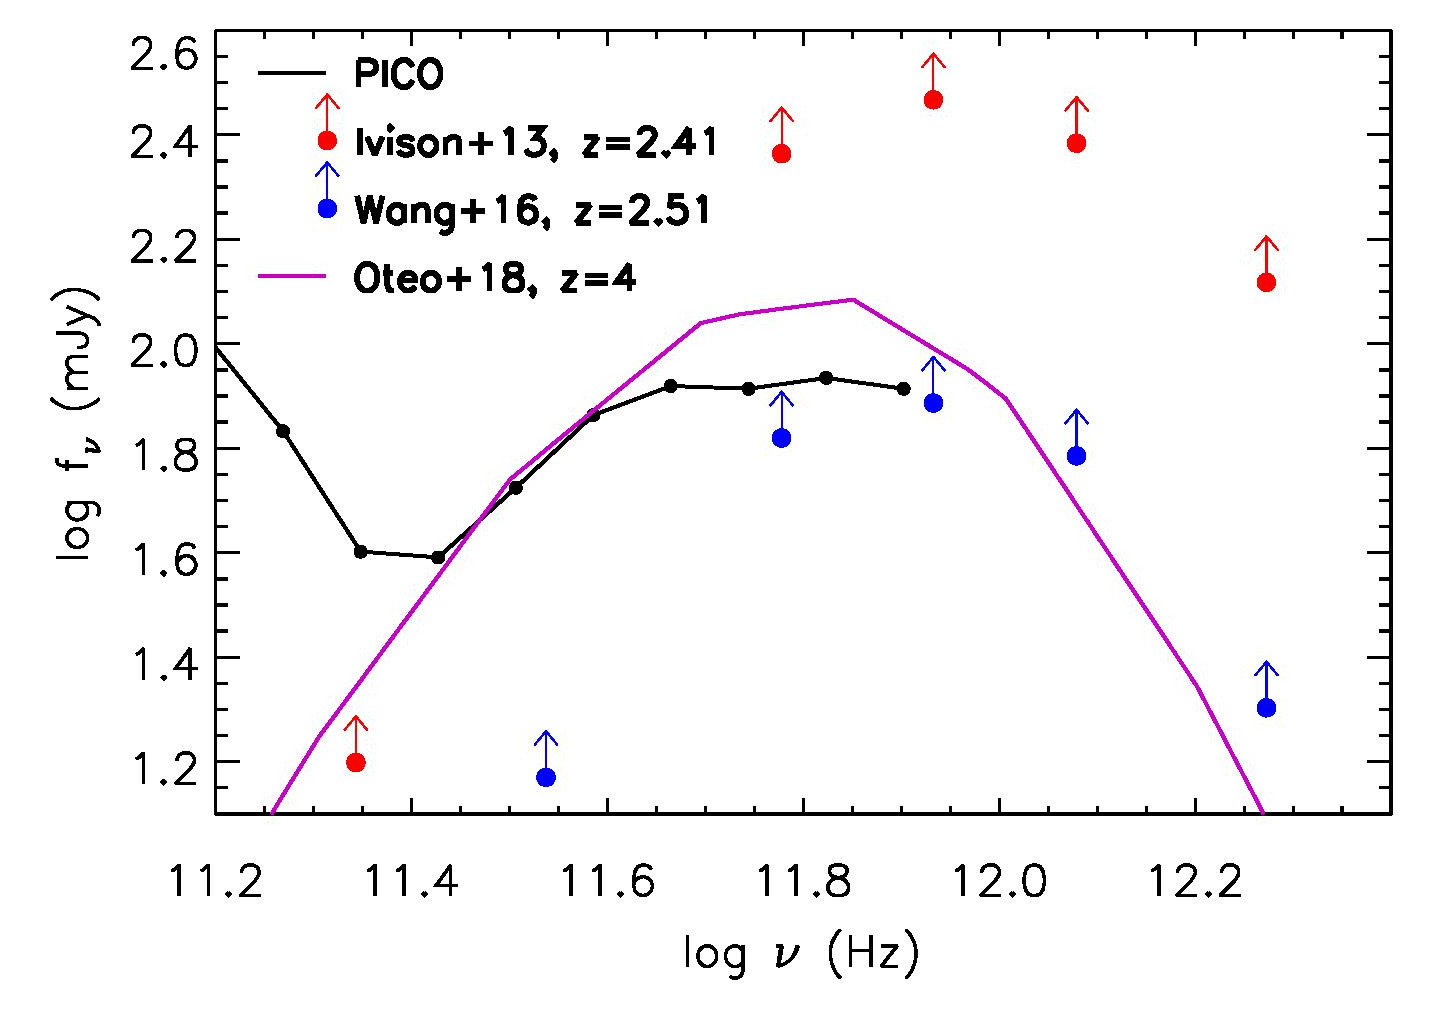
\includegraphics[width=0.32\columnwidth, trim={0 0 0 0cm}, clip]{images/fig_protocl_PICO}
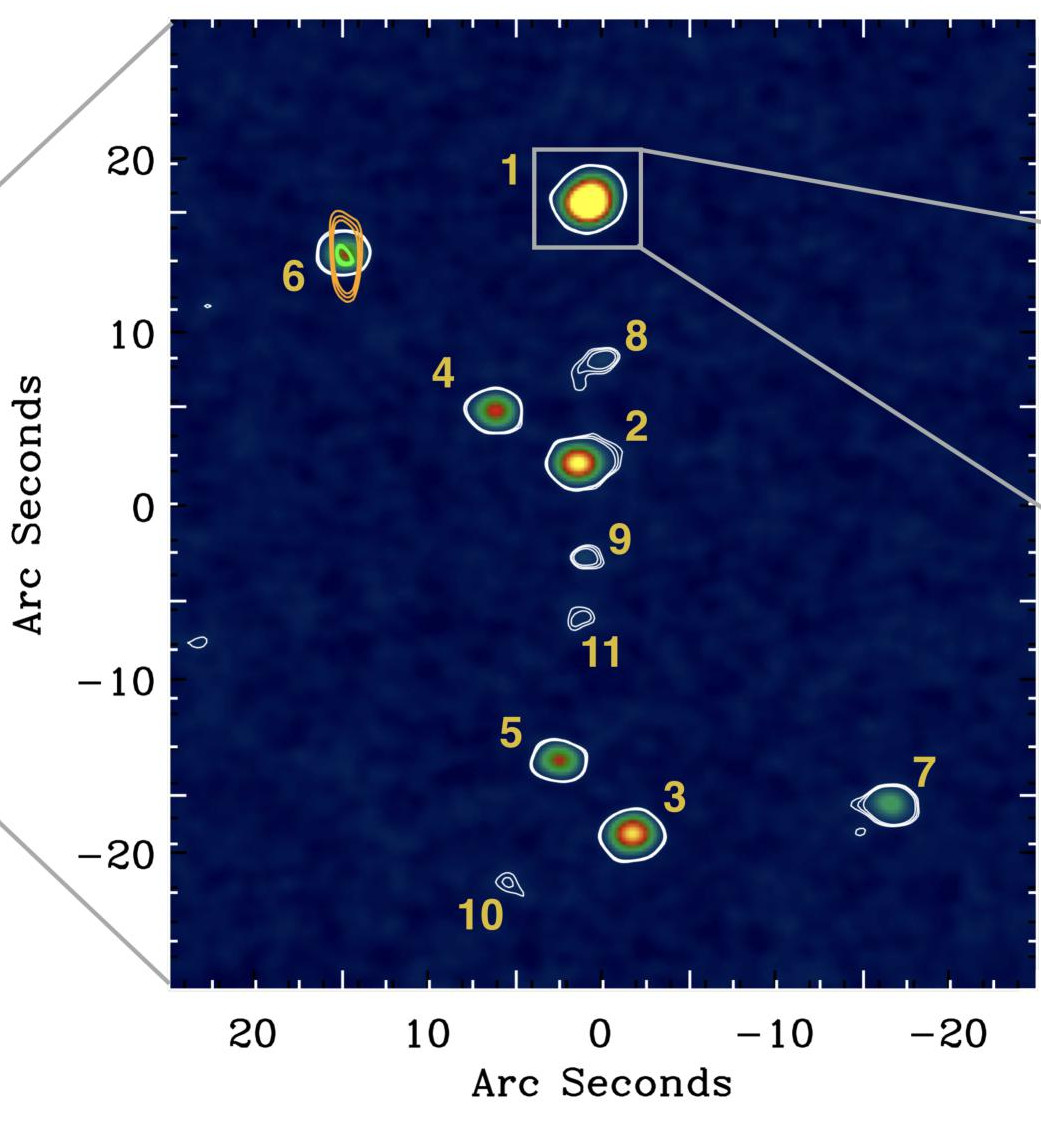
\includegraphics[width=0.32\columnwidth, height=3.7truecm, trim={0 0 0 0.cm}, clip]{images/Oteo_2018_protocl.jpg}
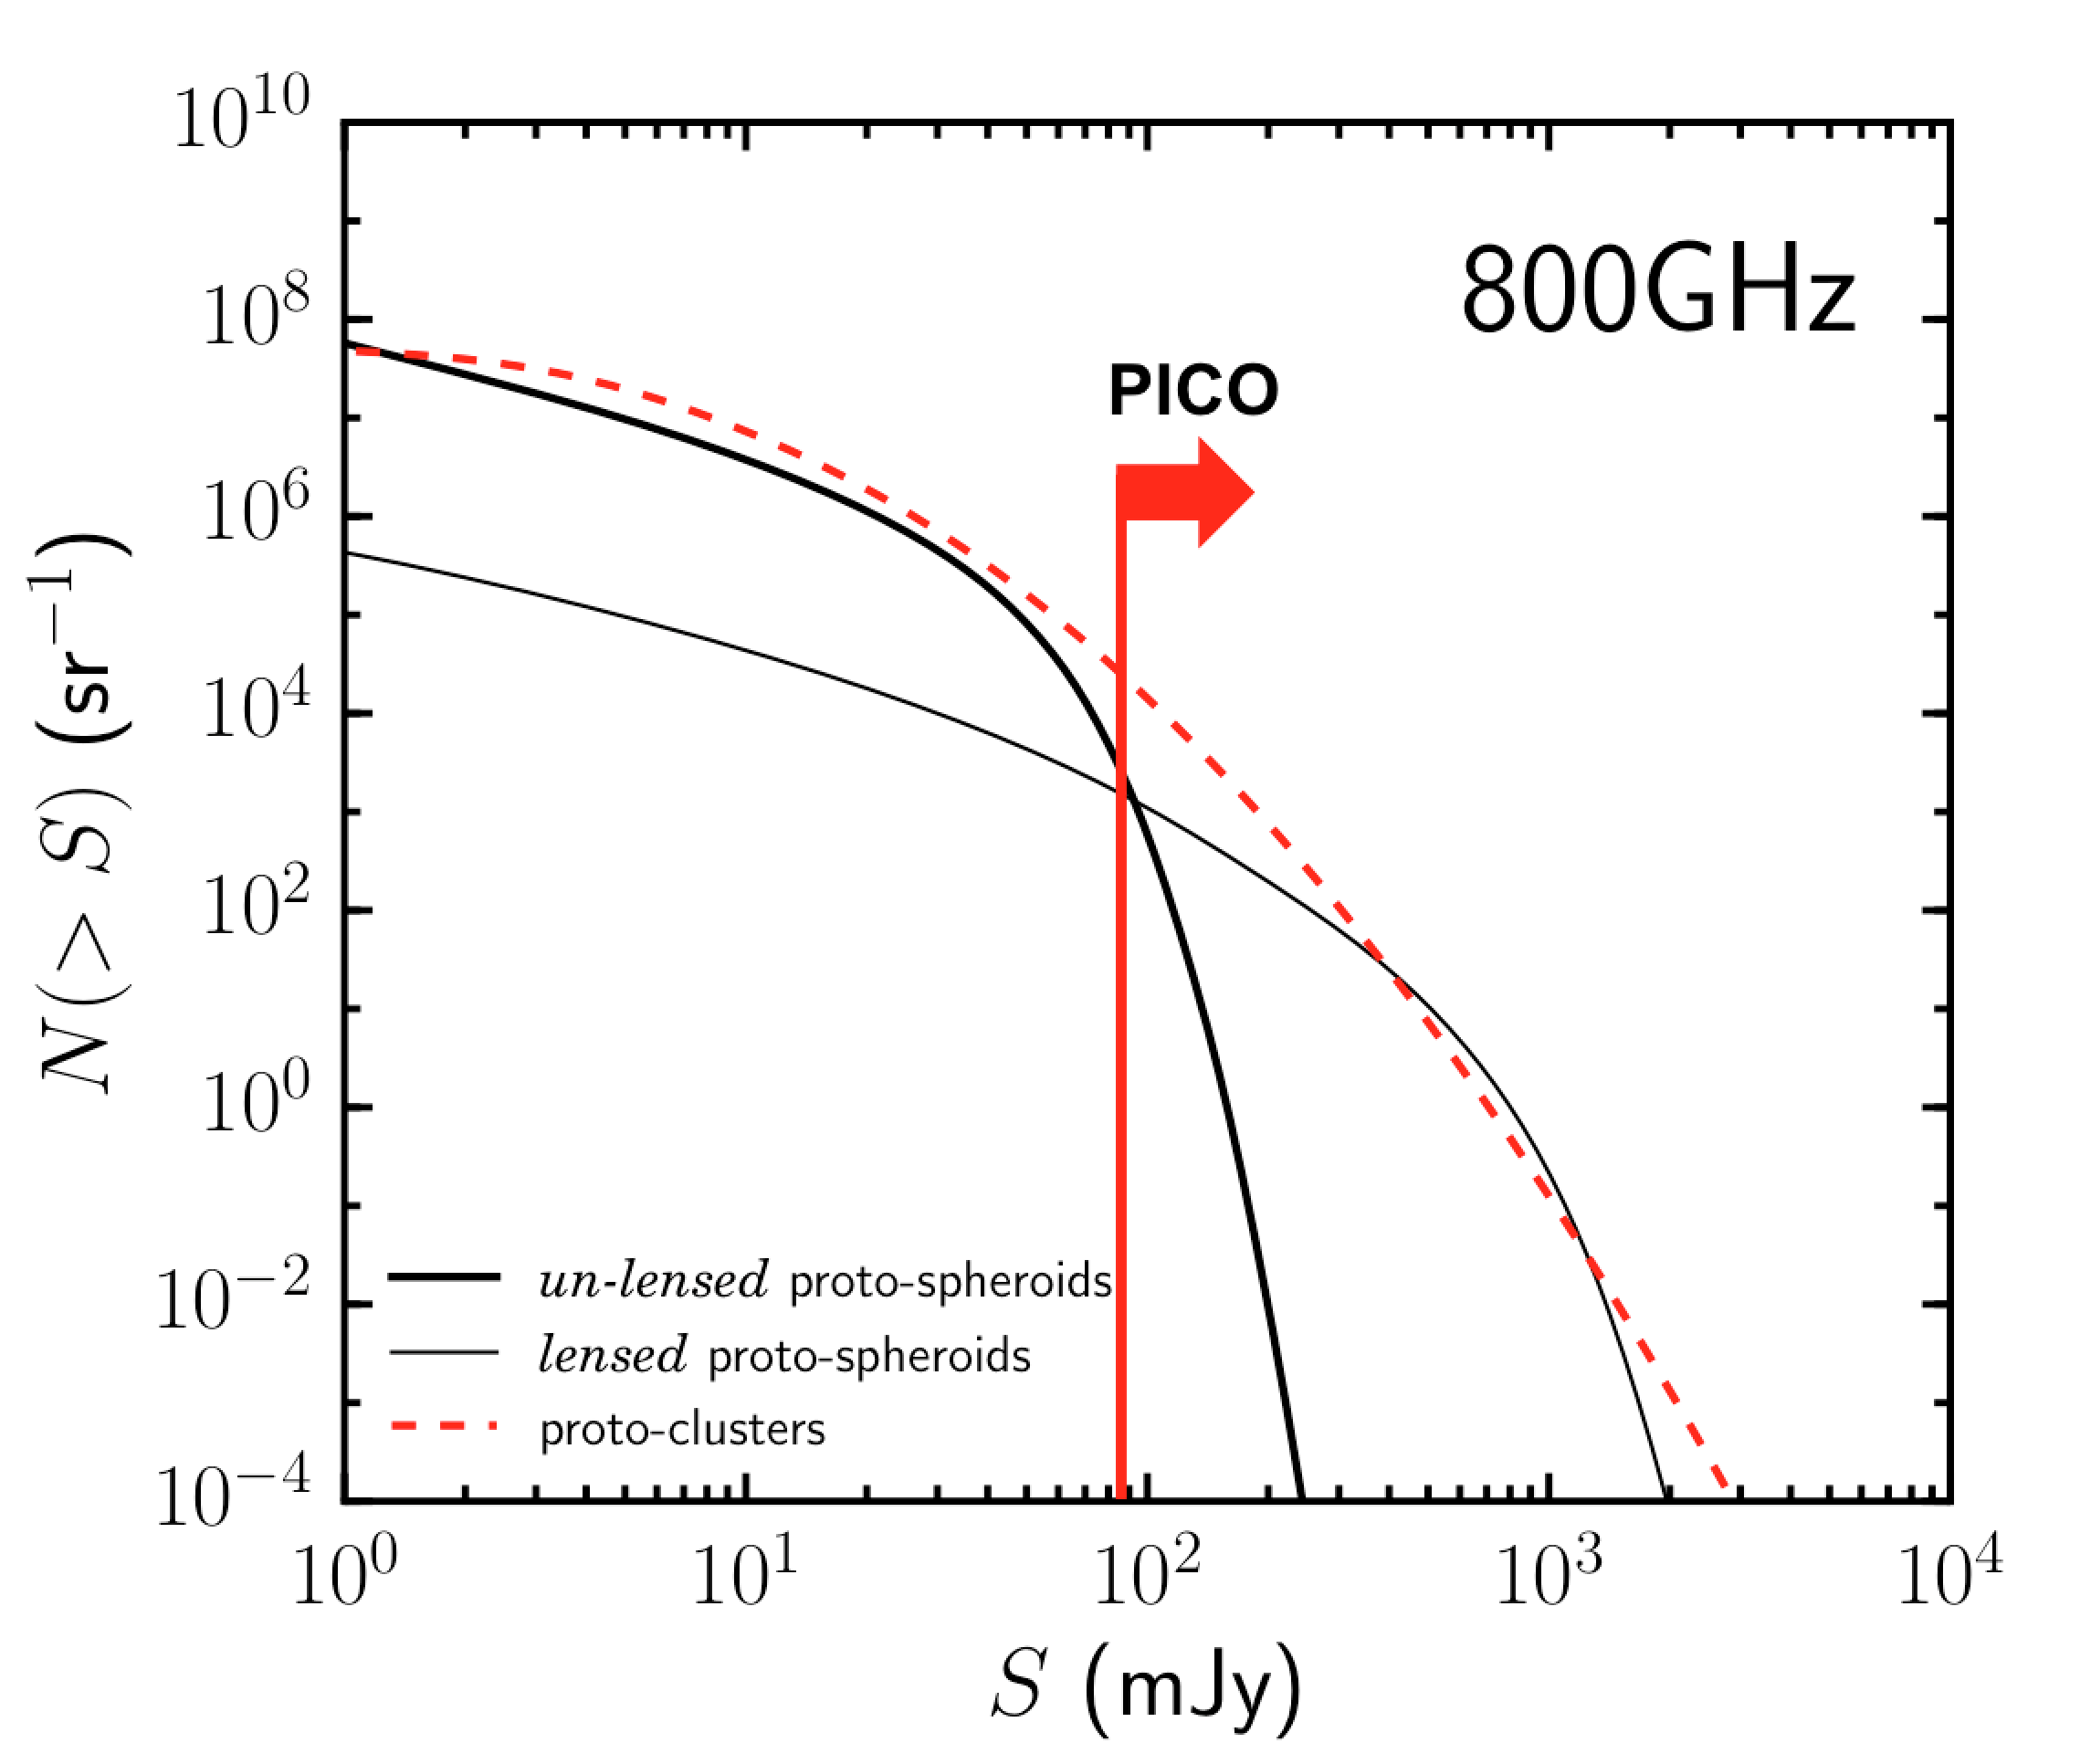
\includegraphics[width=0.32\columnwidth, height=3.7truecm, trim={0 0 0 0.cm}, clip]{images/NgtFclumps_800GHz.png}
%\includegraphics[width=0.48\columnwidth, trim={0 0 0 0.cm}, clip]{dNdzclumps_600GHz.jpg}
\caption{\textbf{Left panel.} SEDs of the cores of two proto-clusters of starbursting galaxies
discovered by \cite{Ivison2013} at $z=2.41$, by \cite{Wang2016} at $z=2.506$ and by \cite{Oteo2018}
at $z=4.0$. The first two SEDs include only the contributions of proto-cluster members within $10''$,
i.e. over an angular size below the PICO resolution, corresponding to physical radii $\simeq 80\,$kpc,
substantially smaller than the effective proto-cluster sizes. The reported flux densities are therefore
lower limits to those that will be measured by PICO. The SED of the $z=4.0$ proto-cluster correspond to
a SFR of $6500\,M_\odot\,\hbox{yr}^{-1}$, estimated by \cite{Oteo2018} summing the contributions of
galaxies detected by ALMA within a radius of $\simeq 25''$; again this is likely a lower limit to what
PICO will measure. The solid black line shows the PICO detection limits.
\textbf{Central panel.} ALMA image of the $z=4.0$ proto-cluster discovered by \cite{Oteo2018}, extracted from Fig.~1 of their paper.
\textbf{Left panel.} Counts of proto-clusters at 800\,GHz predicted by the  model of ref. \cite{Negrello2017protocl}.
The vertical red line corresponds to the PICO detection limit.
%\textbf{Lower right panel.} Predicted redshift distribution of proto-clusters above the PICO detection limit at 800\,GHz.
}
\label{fig:protocluster}
\end{center}
\end{figure*}


\subsubsection{Early phases of cluster evolution}

PICO will open a new window for the investigation of early phases of cluster
evolution,  when their member galaxies were actively star forming and before
the hot IGM was in place. In this phase traditional approaches to cluster
detection (X-ray and SZ surveys, searches for galaxy red sequences) work only
for the minority of evolved objects; indeed they have yielded only a handful of
confirmed proto-clusters at $z\simgt 1.5$ \cite{Overzier2016}\footnote{More
high-$z$ proto-clusters have been found targeting the environment of tracers of
very massive halos, such as radio-galaxies, QSOs, sub-mm galaxies. These
searches are however obviously biased.}.

SEDs of spectroscopically confirmed sub-mm-bright proto-clusters detectable by
PICO  are shown in the left panel of Fig.~\ref{fig:protocluster}).
\textit{Planck} has demonstrated the power of low-resolution surveys for the
study of large-scale structure  \cite{Planck2016high_z} but its resolution was
too poor to detect individual proto-clusters \cite{Negrello2017protocl}. As
illustrated by the central panel of Fig.~\ref{fig:protocluster}, the typical
sizes of high-$z$ proto-cluster cores are of $\sim 1'$ (cf. also ref.
\cite{Alberts2014}), nicely matching the PICO FWHM at the highest frequencies.

CMB Probe will detect many tens of thousands of these objects (right-hand panel
of  Fig.~\ref{fig:protocluster}) up to $z\simgt 4$ (left panel). This will
allow a real breakthrough in the observational validation of the formation
history of the most massive dark matter halos, traced by clusters, a crucial
test of models for structure formation. Follow-up observations will
characterize the properties of member galaxies, probing the galaxy evolution in
dense environments and shedding light on the complex physical processes driving
it.

\subsubsection{Radio sources}

PICO will increase by orders of magnitude the number of blazars selected at
sub-mm  wavelengths and will determine the SEDs of many hundreds of them up to
800\,GHz. The most luminous high-$z$ FSRQs were found to host black holes (BHs)
with the largest masses, up to $\sim 4\times 10^{10}\,M_\odot$ (S$5\,0014+813$,
at  $z = 3.366$; see ref. \cite{Ghisellini2009}). Such objects have
particularly hard mm-wave spectra; thus PICO surveys are well suited to detect
them. Objects like S$5\,0014+813$ are detectable by PICO up to $z>5$.

Blazar searches are the most effective way to sample the most massive BHs at
high $z$ because of the Doppler boosting of their flux densities. Since the
flux boosting occurs for jets closely aligned with the line of sight ($\theta <
1/\Gamma$, $\Gamma \sim 15$ being the bulk Lorentz factor), for each FSRQ there
are other $2\Gamma^2$  (i.e. hundreds) sources of similar intrinsic properties
but pointing elsewhere.

Very large BH masses at high-$z$ challenge models because it is very hard to
grow a seed BH from stellar mass to $> 10^9\,M_\odot$ in the limited age of the
universe. It is even more so for jetted quasars because jets are likely
associated with rapidly spinning BHs whose radiative efficiency is large so
that the mass growth is slow. Yet at least 4 FSRQs has been discovered at $z>5$
(up to $z=5.48$; \cite{Romani2004}). One (SDSS J$013127.34032100.1$ at $z =
5.18$) has estimated BH mass of $\sim 10^{10}\,M_\odot$ \cite{Ghisellini2015}.

The PICO surveys of the largely unexplored mm/sub-mm spectral region will also
offer the possibility to discover new transient sources \cite{Metzger2015} or
events, such as blazar outbursts.

%\begin{figure}
%\vskip-3cm
%\includegraphics[width=\columnwidth]{./COrE_pol_detections_both.png}
%\caption{Comparison of the estimated source number counts in polarization for a selection of CORE channels and different source populations: radio sources (solid blue line); and two populations of dusty galaxies (proto-spheroids and late-type, spiral and starburst, galaxies). Proto-spheroids, labelled ``High-z IR'' (solid green line) dominate at faint flux densities while late-types  (LT IR, solid red lines) dominate at the brighter flux densities. The vertical lines show the $4\sigma$ and  $5\sigma$ detection limits obtained from the simulations for the 1-m ({dashed}) and 1.5-m ({solid}) telescope. From \citet{DeZotti2016}.}
%\label{fig:both}
%\end{figure}

\subsubsection{Source polarization}

PICO will make a giant leap forward in the determination of polarization
properties of both radio sources and of dusty galaxies over a frequency range
where ground based surveys are impractical or impossible. Thanks to its high
sensitivity, it will detect in polarization both populations  over a
substantial flux density range, determining directly, for the first time,
number counts in polarized flux density.

Mm/sub-mm polarimetry of radio sources provides unique information on the
magnetic  field configuration (geometry and degree of order) in the innermost,
unresolved regions of the jets, close to the active nucleus. Polarimetry of
dusty galaxies as a function of their inclination is informative on the
structure and on the ordering of their large-scale magnetic fields.




\end{document}

%\begin{figure}[!htb]
%\centering
%
\includegraphics[width=4cm]{images/example}
%\caption{example}
%\label{fig:im_3}
%\end{figure}
